\section{Assoliment dels objectius}

\subsection{Estudi de l'estat de l'art}
S'ha realitzat un estudi extens de l'estat de l'art, que ha requerit diverses setmanes de recerca i estudi dels avenços més nous en la matèria. S'ha pogut veure com aquest camp avança a un pas imparable i on pràcticament setmanalment apareixen noves solucions per provar. Tant a l'espai \textit{open source} com al privat, s'ha pogut posar a prova les tecnologies més modernes disponibles i valorar els seus avantatges i desavantatges. Es considera que aquest objectiu \textbf{ha sigut assolit satisfactòriament}.

\subsection{Implementació del pipeline}
El \textit{pipeline} ha sigut dissenyat i implementat des de zero, tenint en compte les especificacions i limitacions del projecte. S'ha estudiat i comprès el funcionament intern del sistema de tiquets OTRS i la llibreria PyOTRS i per aconseguir configurar una base de dades amb aquest sistema i extreure els tiquets amb tota la informació necessària. Addicionalment, s'ha escrit una cadena de preprocessament de tiquets per tal de poder obtenir totes les dades en el millor format possible i evitar repeticions o dades irrellevants. S'ha experimentat amb la base de dades \textit{Elasticsearch} per poder inserir informació en una base de dades mitjançant la llibreria requerida. Finalment, no s'ha pogut treballar amb la funció d'anonimització que s'ha mencionat per limitacions externes, però es considera que no és una prioritat que hagi afectat el desenvolupament del projecte. És per això, que es considera que aquest objectiu \textbf{ha sigut assolit satisfactòriament}.

La figura 1 il·lustra el desplegament final de la \textit{pipeline}. Es pot veure com el portàtil amb GPU només s'utilitza per l'execució del model però la resta d'eines s'executen en el seu servidor designat.

\begin{figure}[H]
    \centering
    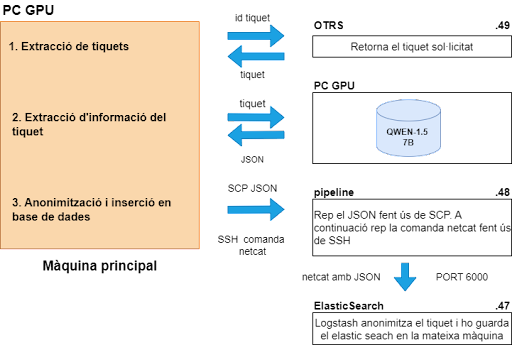
\includegraphics[width=\textwidth]{pipeline_flux_real.png}
    \caption[Pipeline mostra el flux d'execució final]{Pipeline que mostra el flux d'execució final utilitzant el portàtil amb GPU. \\ (Creació pròpia)}
    \label{fig:pipeline_flux_real}
\end{figure}



\subsection{Sistema d'extracció d'informació}
Aquest sistema d'extracció d'informació ha pres forma d'un model del llenguatge natural. Aquest model preentrenat ha sigut entrenat amb la tècnica de \textit{fine-tuning} per aconseguir el millor rendiment possible. Tot i que el projecte ha assolit fites notables, és essencial reconèixer certes limitacions que han repercutit en la seva capacitat per assolir el màxim potencial. Aquestes limitacions són inherents a l'abast del projecte i factors externs que escapen al control. Notablement, per validar encara més l'eficàcia dels resultats obtinguts, seria valuós fer proves amb dades del món real. Aquest pas proporcionaria una representació més precisa dels resultats i demostraria la seva fiabilitat i l'aplicabilitat. Es considera que aquest objectiu \textbf{ha sigut assolit satisfactòriament}.

En conclusió, aquest projecte serveix de base per a un processament de tiquets automàtic. Tot i que la implementació actual utilitza una solució temporal per limitacions de maquinari, demostra l'eficàcia de l'enfocament dissenyat. El treball futur se centrarà a aconseguir un servidor amb els recursos de GPU necessaris i perfeccionar el model NLP per obtenir un rendiment òptim.

\subsection{Desplegament API}
El desplegament de l'API s'ha endarrerit principalment a causa de la manca de temps disponible. Es va prendre la decisió de donar prioritat a totes les altres seccions del projecte per tal de garantir que totes les responsabilitats essencials s'abordessin a temps. Tot i aquest retard, l'equip manté el compromís de completar el desplegament de l'API com més aviat millor, una vegada que la càrrega de treball actual estigui més ben equilibrada. Es considera que aquest objectiu \textbf{no ha sigut assolit}.
